% This work is licensed under the Creative Commons
% Attribution-NonCommercial 3.0 Unported License. To view a copy of this
% license, visit http://creativecommons.org/licenses/by-nc/3.0/.

\section{Aufbau}

Der Versuchsaufbau besteht aus einer Lichtquelle, einer Bank, auf der
die verschiedenen Linsen und der abzubildende Gegenstand gesetzt und
verschoben werden kann, und einem Schirm, auf dem das Bild sichtbar
gemacht wird. Die Bank ist mit einer Scala versehen und erlaubt dadurch
eine Messung der Abstände zwischen den beteiligten Komponenten. Eine
Skizze der Anordnung ist in Abbildung~\ref{fig:aufbau} zu sehen.

\begin{figure}
  \centering
  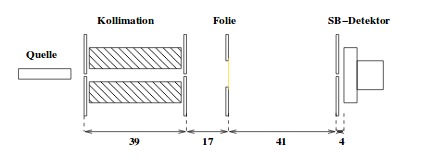
\includegraphics{aufbau}
  \caption{Der Aufbau des Versuchs. Zu sehen ist die Bank, auf der
    Lichtquelle, Perl-L, Linse und Schirm aufgesetzt sind. Linse, Perl-L
    und Schirm lassen sich auf dem Reiter verschieben, wodurch die
    Gegenstands- und Bildweite eingestellt werden kann.}
  \label{fig:aufbau}
\end{figure}
